\subsection{getHostnames}
Request Type: \textbf{GET}
\newline
Request Address: \textbf{/gethostnames}
\newline

This endpoint takes in no data and will return a list of all \textbf{unique} hostnames found among the "run\_information" document embedded in the top level MongoDB documents.

It should be noted that only the documents uploaded using the Adapt uploader script found in ParFlow Performance Testing will have the "run\_information" embedded document field, so this will not return any document information taken from data uploaded using Shweta's uploader script.

\subsubsection{Data Format}
\textbf{Required Data}: \textbf{N/A}
\newline
\newline
\textbf{Returned Data}:
\newline
\newline
This endpoint will return a JSON document with a key/value containing a list of unique hostnames found in the database. An example of what this JSON document looks like can be found in Figure \ref{fig:getHostnames}.

\begin{figure}[H]
    \centering
    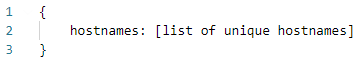
\includegraphics{img/gethostnames.PNG}
    \caption{getHostnames Returned Data Format}
    \label{fig:getHostnames}
\end{figure}
